\chapter{Progettazione}
\label{cap:progettazione}

\intro{Il seguente capitolo ha la funzione di illustrare l'approccio alla progettazione e all'architettura del sistema commissionato.}

\setlength{\parskip}{3ex}

\section{Approccio MDA}
La filosofia dell'azienda per fronteggiare nuove attività e progetti si basa su un approccio di tipo MDA (Model Driven Architecture). L'idea alla base di tale approccio risiede nel fatto che il cuore di ogni applicazione si traduce in un modello solido e ben strutturato. 

\setlength{\parskip}{3ex}

\noindent L'approccio MDA è stato utilizzato anche per affrontare la fase di progettazione del sistema commissionato. In particolare la prima attività è stata quella di definire i modelli su cui l'intero sistema si basa. Per modello si intende un oggetto che deve essere mappato e gestito in una opportuna tabella di un database relazionale.   

\setlength{\parskip}{3ex}

\noindent I modelli vengono rappresentati dalla seguente stringa:

\setlength{\parskip}{2ex}

\noindent \textbf{NomeModello} (TipoAttributo1 nomeAttributo1, ..., TipoAttributoN nomeAttributoN).

\pagebreak

\noindent In particolare i modelli identificati in base alle richieste del committente sono i seguenti:
\begin{itemize}
\item \textbf{Progetto} (Long idProponente, Long idReferente, String codice, String titolo, String descrizione, String statoAvanzamento, Integer giorni, Integer percentualeAvanzamento, GregorianCalendar dataInizio)

\setlength{\parskip}{3ex}

\noindent \textbf{DESCRIZIONE}: questo modello rappresenta un progetto commissionato all'azienda da parte di un cliente o ideato dall'azienda per raggiungere nuovi clienti.

\setlength{\parskip}{3ex}

\noindent \textbf{ATTRIBUTI}:
\begin{itemize}
\item \textit{idProponente} corrisponde all'identificativo del  proponente, ovvero l'azienda da cui nasce l'idea del progetto (CWBI o altro cliente);
\item \textit{idReferente} corrisponde all'identificativo di un dipendente di CWBI che assume il ruolo di responsabile del progetto;
\item \textit{codice} corrisponde ad un identificativo del progetti (es. 2023.70);
\item \textit{titolo} corrisponde al titolo del progetto;
\item \textit{descrizione} corrisponde alla descrizione generale  progetto che illustra l'obiettivo e le funzionalità;
\item \textit{statoAvanzamento} corrisponde allo stato attuale  del progetto. Lo stato può assumere i seguenti valori: {aperto, chiuso, approvato, rifiutato, sospeso};
\item \textit{giorni} corrisponde ai giorni di sviluppo previsti per portare a termine il progetto;
\item \textit{percentualeAvanzamento} corrisponde alla percentuale di avanzamento delle attività di progetto;
\item \textit{dataInizio} corrisponde alla data di inizio delle attività di progetto.
\end{itemize}

\setlength{\parskip}{6ex}

\item \textbf{CorrelazioneProgettoCliente} (Long idCliente, Long idProgetto)

\setlength{\parskip}{3ex}

\textbf{DESCRIZIONE}: questo modello rappresenta la correlazione che persiste tra un progetto e un certo cliente. Si fa notare che uno stesso progetto può raggiungere più di un cliente.

\setlength{\parskip}{3ex}

\textbf{ATTRIBUTI}:
\begin{itemize}
\item \textit{idCliente} corrisponde all'identificativo di un cliente;
\item \textit{idProgetto} corrisponde all'identificativo di un progetto esistente.
\end{itemize}

\pagebreak

\item \textbf{Offerta} (Long idCliente, Long idProgetto, String titolo, String descrizione, String stato, GregorianCalendar dataStipula, BigDecimal imponibile1, BigDecimal imponibile2, BigDecimal imponibile3)

\setlength{\parskip}{3ex}

\textbf{DESCRIZIONE}: questo modello rappresenta l'offerta che viene stipulata per un certo cliente in merito ad uno dei progetti a disposizione.

\setlength{\parskip}{3ex}

\textbf{ATTRIBUTI}:
\begin{itemize}
\item \textit{idCliente} corrisponde all'identificativo di un cliente;
\item \textit{idProgettoCliente} corrisponde all'identificativo di un progetto esistente;
\item \textit{titolo} corrisponde al titolo dell'offerta (es. Contratto n.7/2023);
\item \textit{descrizione} corrisponde alla descrizione dell'offerta emessa (note, informazioni utili, ecc.);
\textit{stato} corrisponde allo stato attuale dell'offerta. Lo stato può assumere i seguenti valori: in preparazione, in accettazione, accettata;
\item \textit{dataStipula} corrisponde alla data in cui l'offerta è stata emessa;
\item \textit{imponibile1} corrisponde al primo prezzo proposto per firmare l'offerta;
\item \textit{imponibile2} corrisponde al secondo prezzo proposto per firmare l'offerta;
\item \textit{imponibile3} corrisponde al terzo prezzo proposto per firmare l'offerta.
\end{itemize}
\end{itemize}

\setlength{\parskip}{6ex}

\noindent I modelli \textbf{Cliente} e \textbf{Utente}, necessari per realizzare il progetto commissionato, erano già stati definiti per un altro modulo dell'applicazione CW GEST. In particolare questi modelli rappresentano rispettivamente un cliente e un dipendente di CWBI. Dato che tali modelli presentano le medesime caratteristiche pensate per il progetto in questione non si è reso necessario alterarli per l'utilizzo.

\pagebreak

\section{Architettura MVC}
Come citato in precedenza, il framework Apache Struts mette a disposizione un'architettura \textbf{MVC} (Model View Controller) per costruire applicazioni web. \\
L'architettura di Struts non si differenzia particolarmente dalla filosofia di MVC: il controller gestisce tutte le operazioni della webapp e ha un riferimento sia al modello sia alla vista. 

\setlength{\parskip}{3ex}

\noindent L'architettura MVC messa a disposizione da Apache Struts viene rappresentata dal seguente schema:

\begin{figure}[!h]
	\centering
	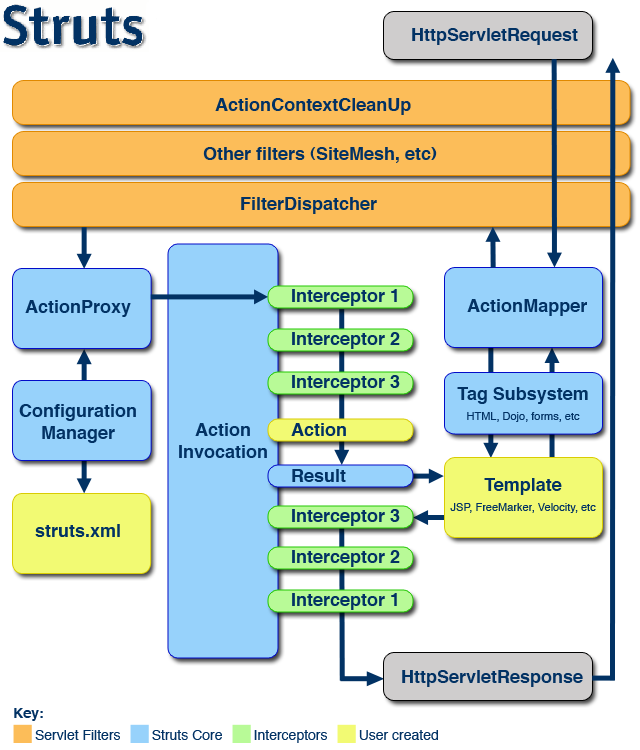
\includegraphics[width=9cm]{../images/MVC.png}
	\caption{Architettura MVC di Apache Struts}
	\label{fig:MVC}
\end{figure}

\setlength{\parskip}{3ex}

\noindent I tre componenti principali della filosofia MVC corrispondo a:
\begin{itemize}
\item \textbf{FilterDispatcher} (Controller);
\item \textbf{Action} (Model);
\item \textbf{Template} (View).
\end{itemize}

\noindent Come si può notare dalla {\hyperref[fig:MVC]{figura 5.1}}, l'architettura offerta dal framework è caratterizzata da diversi componenti che risulta necessario menzionare per apprendere a fondo il pieno funzionamento del sistema MVC di Apache Struts. Questi componenti sono i seguenti: 

\begin{itemize}
\item \textbf{FilterDispatcher}: rappresenta il controller del framework ed è il primo componente ad agire nel ciclo di elaborazione della richiesta. Il controller ispeziona ogni richiesta in arrivo per determinare quale action dovrebbe gestire la richiesta.
\setlength{\parskip}{3ex}

\item \textbf{Action}: rappresenta una funzione dell'applicativo ed è qui che viene definita la logica applicativa del sistema.\\
In particolare ogni modello è caratterizzato da n action che gestiscono le funzionalità che devono essere garantite all'utente (es. una action per la pagina di dettaglio, una per la creazione/modifica dell'oggetto, una per la ricerca dell'oggetto attraverso dei filtri, ecc.).
\setlength{\parskip}{3ex}

\item \textbf{ActionMapper}: viene utilizzata da FilterDispatcher per determinare se la richiesta deve richiamare una action o meno. Quando viene fornito un HttpServletRequest, ActionMapper può restituire null se nessuna action corrisponde alla richiesta  oppure può restituire un ActionMapping che descrive la chiamata.

\setlength{\parskip}{3ex}

\item \textbf{ActionProxy}: se ActionMapper determina che deve essere richiamata una action per tale richiesta, FilterDispatcher delega il controllo ad ActionProxy. L'ActionProxy si consulta con ConfigurationManager, un'interfaccia che descrive la configurazione del framework, e crea una ActionInvocation che si occupa di richiamare l'opportuna action che deve gestire la richiesta entrante.
\setlength{\parskip}{3ex}

\item \textbf{Interceptor}: corrispondono a dei componenti che vengono richiamati prima di eseguire la action e hanno il compito di preparare e inizializzare le action stesse.
\setlength{\parskip}{3ex}

\item \textbf{Result}: corrisponde al risultato costruito e ritornato dalla action e che viene rappresentato da una pagina JSP.
\setlength{\parskip}{3ex}

\item \textbf{Template}: corrispondono alle pagine di visualizzazione che effettivamente restituiscono la risposta all'utente.
\setlength{\parskip}{3ex}

\end{itemize}

\pagebreak

\noindent Il ciclo che parte da una richiesta entrante risulta essere il seguente:
\begin{enumerate}
\item la richiesta viene raccolta da ActionMapper;

\item viene chiamato il filtro FilterDispatcher che consulta ActionMapper per determinare se un'azione deve essere richiamata;

\item se ActionMapper trova che un'azione deve essere richiamata, FilterDispatcher delega il controllo ad ActionProxy;

\item ActionProxy legge il file di configurazione (struts.xml). ActionProxy crea un'istanza della classe ActionInvocation e delega il controllo.

\item ActionInvocation gli Interceptor uno per uno (se richiesto) e quindi invoca la action;

\item la action ritorna il risultato, gli Interceptor vengono eseguiti nuovamente in ordine inverso e la risposta viene restituita a FilterDispatcher;

\item Il risultato viene quindi inviato al contenitore servlet che a sua volta lo rispedisce al client.
\end{enumerate}

\pagebreak
